\documentclass[10pt,a4paper]{article}
\usepackage[margin=20mm]{geometry}
\usepackage[T1]{fontenc}
\usepackage{graphicx,longtable,booktabs}
\usepackage[hidelinks]{hyperref}
\title{WindCtrl Validator\\\large Controller Validation Report}
\author{Engineering demonstration}
\date{}
\begin{document}
\maketitle
\section*{Scope and assumptions}
Offline row-level validation of simulated or user-supplied test records.
This is an independent portfolio project, not a turbine certification tool.
Demonstration limits are configurable and are not manufacturer specifications.
Controller output is interpreted as a power command in kW. Each record is
checked for data validity, range, state consistency, temperature and tracking error.
\section*{Configuration}
Power and controller tolerance: 5.0\%. Zero-demand absolute tolerance: 0.5 kW.
Maximum generator temperature: 100.0 degrees C. Boundaries are inclusive.
\section*{Validation summary}
\begin{tabular}{lr}\toprule Metric & Value \\ \midrule
Total Tests & 360 \\
Passed Tests & 323 \\
Failed Tests & 37 \\
Pass Pct & 89.72 \\
Average Error Pct & 1.6019 \\
Maximum Error Pct & 12.0 \\
Maximum Deviation Kw & 240.0 \\
Percentage Comparable Rows & 357 \\
\bottomrule\end{tabular}
\paragraph{Metric denominator.} Percentage error excludes zero or invalid expected
power and invalid observed power. Sensor failures remain included when power
values are valid. Zero-demand records use absolute error; consult the comparable
row count. Maximum deviation in kW includes valid zero-demand comparisons.
\section*{Engineering plots}
\IfFileExists{validation.png}{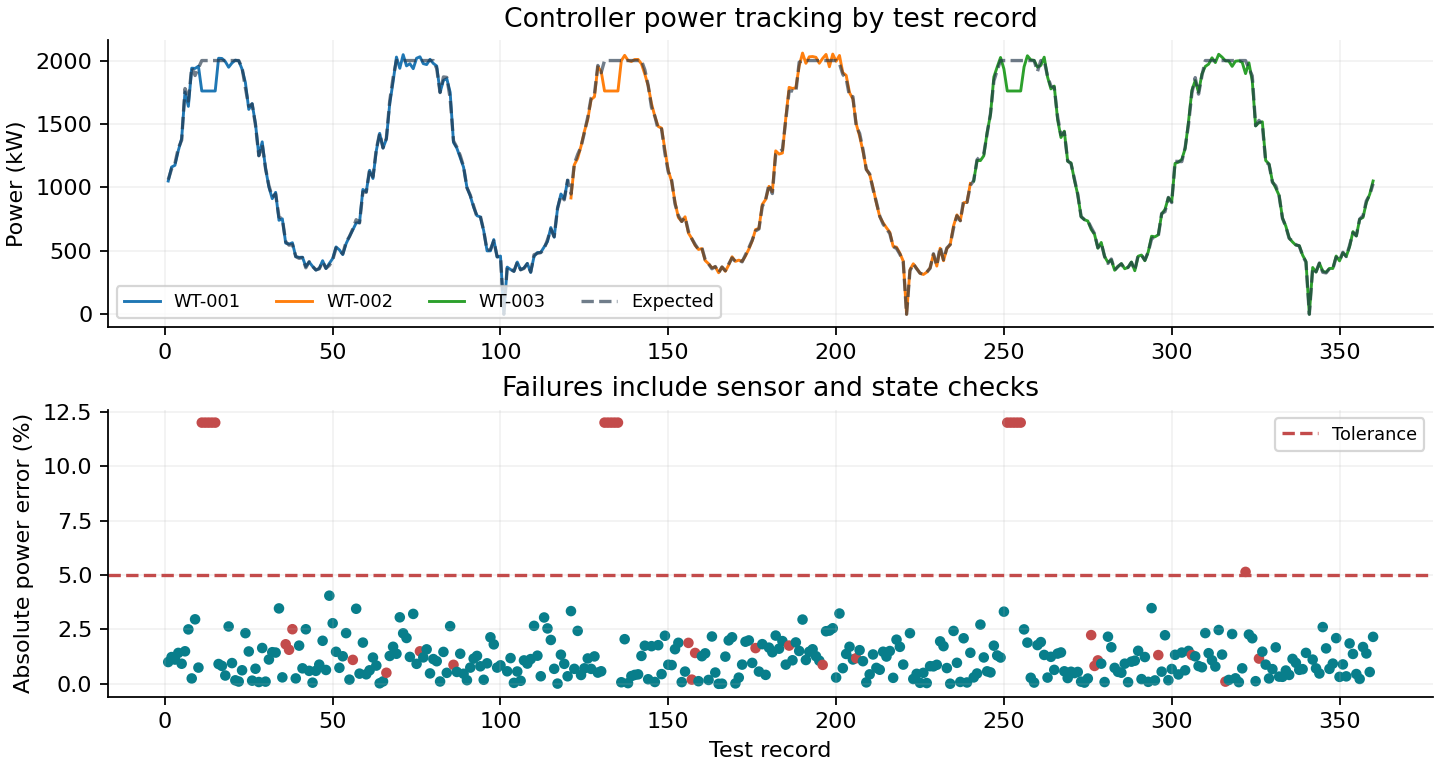
\includegraphics[width=\linewidth]{validation.png}}{Plot unavailable.}
\section*{Failure detail (first 20)}
\begin{longtable}{r p{20mm} p{110mm}}\toprule ID & Turbine & Reasons \\ \midrule
11 & WT-001 & power deviation exceeds tolerance \\ \hline
12 & WT-001 & power deviation exceeds tolerance \\ \hline
13 & WT-001 & power deviation exceeds tolerance \\ \hline
14 & WT-001 & power deviation exceeds tolerance \\ \hline
15 & WT-001 & power deviation exceeds tolerance \\ \hline
36 & WT-001 & generator over-temperature \\ \hline
37 & WT-001 & generator over-temperature \\ \hline
38 & WT-001 & generator over-temperature \\ \hline
56 & WT-001 & wind\_speed\_mps: missing or non-finite number \\ \hline
66 & WT-001 & unexpected controller state; positive demand requires RUNNING state \\ \hline
76 & WT-001 & rotor\_speed\_rpm: outside demonstration range [0, 30] \\ \hline
86 & WT-001 & controller deviation exceeds tolerance \\ \hline
131 & WT-002 & power deviation exceeds tolerance \\ \hline
132 & WT-002 & power deviation exceeds tolerance \\ \hline
133 & WT-002 & power deviation exceeds tolerance \\ \hline
134 & WT-002 & power deviation exceeds tolerance \\ \hline
135 & WT-002 & power deviation exceeds tolerance \\ \hline
156 & WT-002 & generator over-temperature \\ \hline
157 & WT-002 & generator over-temperature \\ \hline
158 & WT-002 & generator over-temperature \\ \hline
\bottomrule\end{longtable}
Full results: \texttt{validation\_results.csv}. Structured metrics:
\texttt{summary.json}. The application does not model controller dynamics,
transient response, interlocks or hardware-in-the-loop behaviour.
\end{document}
